% MediSense-Cardio -- journal manuscript (Physiological Measurement, IOP). DRAFT scaffold, 2026-09-25.
%
% Written as a plain `article` so it compiles anywhere. Before submission, port to IOP's `iopart` template
% (optional per IOP) and switch the bibliography to Harvard author-year (IOP requires Harvard for this journal).
% Body text is split into sections/*.tex. Anything not yet verified or still pending is marked with \pending{...}
% (red) so it cannot be missed. Numbers come from scripts/analysis/*.py and docs/journal/tables/*.csv.

\documentclass[11pt,a4paper]{article}
\usepackage[margin=2.3cm]{geometry}
\usepackage[T1]{fontenc}
\usepackage{lmodern,microtype}
\usepackage{amsmath,amssymb}
\usepackage{graphicx,booktabs,array,tabularx,longtable}
\usepackage{xcolor}
\usepackage[authoryear,round]{natbib}
\usepackage{url}
\usepackage{setspace}
\usepackage[hidelinks]{hyperref}
\usepackage{caption}
\captionsetup{font=small,labelfont=bf}
\setstretch{1.1}

\newcommand{\pending}[1]{\textcolor{red}{\textbf{[PENDING: #1]}}}
\newcommand{\todo}[1]{\textcolor{red}{\textbf{[TODO: #1]}}}
\newcommand{\bpm}{\,bpm}
\newcommand{\ms}{\,ms}

\title{From a photographed paper ECG to what a patient is told: a step-by-step, reproducible study of how image degradation propagates through an open-source digitisation pipeline\\[2pt]
\large\textit{[working title -- confirm with the guide]}}
\author{\todo{author names, affiliations, corresponding author e-mail}}
\date{}

\begin{document}
\maketitle

\begin{abstract}
\noindent\textbf{Objective.} To quantify how deliberate image degradation of a photographed paper ECG propagates through an open-source digitisation pipeline into heart-rate and interval measurements, to test whether it produces falsely reassuring results, and to document the workflow reproducibly.

\noindent\textbf{Approach.} Fifty PTB-XL records (25 normal, 25 abnormal) were rendered as printed ECG pages, degraded along six axes (blur, tilt, JPEG compression, resolution, uneven lighting, grid contrast) at five levels each, digitised with Open-ECG-Digitizer, and compared with ground truth: 1{,}550 tests per sweep, in two sweeps five days apart. We measured heart rate, PR, QRS, QT and QTc, with paired tests (Holm correction) and Bland--Altman analysis.

\noindent\textbf{Main results.} On clean images the heart-rate bias was $+0.26$\bpm\ (95\% limits $-3.1$ to $+3.6$). Only blur and low resolution produced large error growth: the median QTc error rose from 17\ms\ to 91\ms\ (blur) and 73\ms\ (resolution) at level~5, and the median heart-rate error from 0.13 to 1.7 and 2.5\bpm. Falsely reassuring heart-rate readings occurred only at level~5 of these two axes, and were identical in a repeat sweep (a computational repeat, not an independent replication). Tilt caused unreadable pictures rather than wrong values. Interval measurement had a clean-image error floor of 11--22\ms, partly due to a 100\,Hz ground truth; a QTc analogue of false reassurance was weak and not concentrated. The digitiser was not version-pinned, and seven records changed readability between sweeps.

\noindent\textbf{Significance.} Quality safeguards for photographed-ECG tools can target blur and low resolution. The workflow, including negative and corrected findings, is documented for reproduction.

\medskip
\noindent\textbf{Keywords:} electrocardiogram; ECG digitisation; image degradation; signal quality; false reassurance; reproducibility
\end{abstract}


\tableofcontents
\newpage

\section{Introduction}

\subsection{Background}
An electrocardiogram (ECG) recorded in a clinic is normally read by trained staff on calibrated equipment. Increasingly, people meet a printed or photographed ECG outside that setting: a printout from a home device, a photograph of a clinic report sent through a messaging application, or an image uploaded to a health application that promises to read it back into numbers and explain them. Reading a paper ECG back into a digital waveform is now technically mature. Open-source tools report signal-to-noise ratios of roughly 20\,dB on real scanned pages \citep{ref5}, an international challenge has benchmarked digitisation methods \citep{ref2}, and purpose-built toolkits can render realistic printed ECG pages from digital signals for controlled testing \citep{ref1}.

What is much less well characterised is how such a pipeline behaves when the input is a poor photograph. Digitisers are normally validated on clean, well-scanned images. A patient's own photograph may be out of focus, tilted, low-resolution, over-compressed, unevenly lit or printed faintly. If the digitised heart rate or interval is wrong because the picture was poor, and the tool reports it with the same confidence as a good one, a downstream statement to the patient can be wrong in the most harmful direction: an abnormal reading described as normal. We call this \emph{false reassurance}. A safeguard against it can only be designed if we know \emph{which} kinds of image degradation produce it, and how severe they must be.

\subsection{Objective}
This paper asks: \emph{how does controlled degradation of a photographed paper ECG propagate through an open-source digitisation pipeline into clinically meaningful measurements, and at what severity, for which degradations, does it produce a falsely reassuring result?} We answer it with a simulation study on public data in which the ground truth is known exactly.

\subsection{What this paper contributes}
\begin{enumerate}
\item A \textbf{complete, step-by-step account} of the study from an empty computer to the final analysis, with the real output of every step (Section~\ref{sec:methods}, Section~\ref{sec:results}), including the dead ends, the bugs and the corrections. The aim is that another group can repeat it.
\item A \textbf{controlled measurement} of six degradation axes at five severities each over 1{,}550 tests, repeated in a second sweep (a computational repeat, not an independent replication), reporting heart rate, PR, QRS, QT and QTc against ground truth with paired statistics.
\item A \textbf{patient-facing outcome analysis}: whether the digitised value would move a patient across a clinical boundary, for heart rate and (more cautiously) QTc.
\item \textbf{Two methodological findings} that matter beyond this study: interval measurements from a reconstructed signal carry a much larger error floor than heart rate, part of which is an artefact of ground-truth sampling rate; and an unpinned digitiser dependency changed which records failed between two runs five days apart.
\end{enumerate}

\subsection{What this paper does not claim}
The project this study belongs to was conceived as a full system: digitise, extract measurements, explain them to the patient in plain language behind a safety boundary, and deliver this through a web application. \textbf{Only the first part has been built and measured.} The explanation, safety-boundary and application stages were deferred and are not evaluated here; they appear only as future work. We also do not claim a diagnostic tool, a validated clinical threshold, or performance on real photographs (Section~\ref{sec:limitations}).

\subsection{Organisation}
Section~\ref{sec:related} places the work in the literature. Section~\ref{sec:methods} describes the data, the software environment and each step of the pipeline, in the order in which it was built. Section~\ref{sec:results} reports the output of each step. Sections~\ref{sec:discussion} and~\ref{sec:limitations} interpret the findings and state their limits.

\section{Related work}\label{sec:related}

We review four bodies of work this study sits between. The review is based on the sources listed in the reference list, compiled and checked between July and August 2026; it is a directed review, not a systematic one, and the statements of novelty below are made in that light.

\subsection{Digitisation of paper and photographed ECGs}
Early digitisation methods used classical image processing to remove the grid, threshold the trace and rescale pixels to millivolts \citep{ref6,ref7,ref8,ref9}. Recent work uses deep networks for trace segmentation and layout recognition \citep{ref10,ref11}. The open-source Open-ECG-Digitizer \citep{ref5}, used here, combines a segmentation network with a lead-name network and a layout-matching step, and reports validation on more than 37{,}000 images. ECGtizer \citep{ref3} and the entry that won the 2024 George B.\ Moody PhysioNet Challenge \citep{ref53} are independent alternatives; the Challenge established signal-to-noise ratio against ground truth as its standard accuracy measure \citep{ref2}. ECG-Image-Kit \citep{ref1} generates realistic printed ECG pages, optionally with artefacts, from digital records, and ECG-image-database \citep{ref4} provides paired images and signals with real-world artefacts such as perspective skew, wrinkles, stains and uneven lighting. Performance on photographs is markedly lower than on scans: Open-ECG-Digitizer reports 19.65\,dB on scans but about 12.2 and 10.5\,dB on two phone cameras \citep{ref5}, and the Challenge winner, at 12.15 on the scans-only leaderboard, scored negative signal-to-noise ratio on the mobile-phone photographs of the hidden set \citep{ref53}. Two recent studies are closest to ours: one benchmarks digitisers separately for each of nine capture or damage types of a Challenge dataset and reports signal-to-noise ratio only \citep{ref54}; the other adds a quality-assurance module after digitisation and scores it on reconstruction fidelity, not clinical error \citep{ref55}. We differ in grading each damage type over five severities, in measuring clinical values rather than signal-to-noise ratio, and in defining and counting false reassurance. We use ECG-Image-Kit for rendering and treat the digitiser as a component under test, not a contribution, and not as a solved problem for phone photographs.

\subsection{Signal and image quality assessment}
A separate literature asks whether an ECG is good enough to analyse at all. Deep classifiers separate interpretable from non-interpretable recordings with high reported accuracy \citep{ref12}, and the problem has been studied for wearable and portable devices \citep{ref13,ref15,ref16,ref19,ref20}, for false-alarm reduction \citep{ref17,ref18}, with unsupervised learning \citep{ref14,ref21} and with attention networks \citep{ref22}. Signal-quality gating before analysis of a \emph{waveform} is therefore feasible and established. The Challenge organisers likewise observe that signal-to-noise ratio does not directly reflect the clinical measurements that influence ECG interpretation \citep{ref2}. That observation motivates the present focus on error at the level of the extracted clinical value.

\subsection{Uncertainty, abstention and deferral}
When should an automated medical system decline to answer? Uncertainty-aware abstention has been studied for medical text \citep{ref23}, conformal and cost-aware deferral for clinical triage \citep{ref24,ref27}, guided deferral for language-model systems \citep{ref25}, uncertainty quantification for ECG interpretation \citep{ref30,ref31}, selective classification for prehospital risk prediction \citep{ref32}, and uncertainty estimation in other diagnostic settings \citep{ref28,ref29}. A cautionary result is that abstention is not automatically safer: when an artificial-intelligence system abstains, clinicians' error patterns shift, with false positives falling and false negatives rising \citep{ref26}. This body of work presupposes an uncertainty estimate; it does not, in the sources we reviewed, connect that estimate to a measured rate of a specific harm caused by a specific, controllable input condition.

\subsection{Patient-facing explanation and medical AI safety}
Language models are increasingly used to translate clinical output into patient-readable text, and their quality and safety have been evaluated for cardiology procedures \citep{ref33}, radiology reports \citep{ref38}, personalised plain-language summaries \citep{ref34}, chronic-disease self-management \citep{ref39} and general patient questions \citep{ref40,ref41,ref42,ref43}. A clinical-safety benchmark defines 30 metrics for medical language models \citep{ref35}. ECG-specific language-model work exists \citep{ref36,ref37} but targets clinicians interpreting a trace, not a patient reading an explanation of their own photograph.

\subsection{Gap}
Each thread stops at a boundary: digitisation stops at the signal, quality assessment at whether the signal is usable, abstention at an assumed uncertainty score, and patient-facing generation at the text. In the sources we reviewed, none measures how far a \emph{controllable image degradation} propagates into a \emph{clinically meaningful measurement} and at what severity it becomes a falsely reassuring one. That measurement is the subject of this paper. It is a necessary input to any later safeguard, whether an upload-time quality gate or an uncertainty-qualified explanation.

\section{Methods}\label{sec:methods}

The study was built in ten steps (Table~\ref{tab:steps}). We describe them in the order in which they were carried out, because several design decisions only make sense as responses to what an earlier step revealed. Section~\ref{sec:results} reports the output of each step under the same numbering.

\begin{table}[ht]
\centering\small
\caption{The ten steps of the study, and where each is described and reported.}\label{tab:steps}
\begin{tabularx}{\textwidth}{@{}c>{\raggedright\arraybackslash}p{5.2cm}>{\raggedright\arraybackslash}X@{}}
\toprule
Step & What was done & Real output shown \\
\midrule
0 & Data selection and sampling & Sample composition (Table~\ref{tab:sample}) \\
1 & Feasibility spike with a stand-in renderer & Recovered fraction of record, beats found \\
2 & Official rendering tool on a real record & Rendered page; layout-match score; heart rate \\
3 & Six-record validation & Table~\ref{tab:step3}, Fig.~\ref{fig:step3} \\
4 & Degradation model & Fig.~\ref{fig:grid}, Table~\ref{tab:degradation} \\
5 & Harness and pilot (10 records, blur) & Throughput; error vs blur; one bug \\
6 & Sweep 1: 1{,}550 tests, checkpointed & Cleaning table; reliability (Fig.~\ref{fig:fig3}) \\
7 & Sweep 1 analysis: heart rate and outcomes & Figs.~\ref{fig:fig1}--\ref{fig:fig2} \\
8 & Sweep 2: PR, QRS, QT, QTc & Completion; data dictionary \\
9 & Sweep 2 analysis and cross-checks & Figs.~\ref{fig:ba}--\ref{fig:intervals}, Tables~\ref{tab:intervals}--\ref{tab:tests} \\
\bottomrule
\end{tabularx}
\end{table}

\subsection{Step 0: data and sampling}
\textbf{Data.} We used PTB-XL v1.0.3 \citep{ref45}, a public 12-lead ECG dataset of 21{,}799 ten-second records from 18{,}869 patients, released under CC-BY 4.0 with diagnostic annotations. The low-resolution (100\,Hz) files were used for rendering and for the sweeps; the 500\,Hz files were used only for the ground-truth sampling-rate check in Section~\ref{sec:gt500}.

\textbf{Labels.} Each record's diagnostic superclass was taken from its highest-likelihood SCP code, mapped through the dataset's statement table. A record was labelled \emph{abnormal} if it had a superclass other than NORM, and \emph{normal} otherwise. One sampled record has a dominant code with no diagnostic superclass and is therefore counted as normal by this rule (Table~\ref{tab:sample}).

\textbf{Sampling.} Because false reassurance can only be observed on a record whose truth is abnormal, sampling was stratified. A pool of 500 records (250 normal, 250 abnormal) was drawn with a fixed random seed (42) and saved; the study sample is a fixed 50-record subset of that pool (25 normal, 25 abnormal, seed 42). \textbf{The sample size was reduced from a planned $\approx$500 records to 150 and then to 50} because 500 records $\times$ 31 versions was estimated at $\approx$87 GPU-hours, which did not fit the free GPU quota or the project deadline; 50 records was estimated at $\approx$10.5 hours. This reduction was decided before any result was seen. The pool, seed and selection code are fixed so the sample can be regenerated exactly (the analysis script reconstructs it from the public metadata).

\begin{table}[ht]
\centering\small
\caption{Composition of the 50-record sample. Sex and age from PTB-XL metadata.}\label{tab:sample}
\begin{tabular}{@{}lr@{\qquad}lr@{}}
\toprule
Diagnostic superclass & Records & Attribute & Value \\
\midrule
NORM & 24 & Male / female & 24 / 26 \\
HYP (hypertrophy) & 9 & Median age (years) & 63 \\
STTC (ST/T change) & 7 & Age range (years) & 26 to $>$89$^{\dagger}$ \\
CD (conduction disturbance) & 5 & Labelled normal / abnormal & 25 / 25 \\
MI (myocardial infarction) & 4 & & \\
No superclass & 1 & & \\
\bottomrule
\end{tabular}

\smallskip
\footnotesize $^{\dagger}$PTB-XL stores ages above 89 as 300 to protect identity; one sampled patient carries that code, and it is not an age.
\end{table}

\subsection{Software environment and its limits}
Development was done on a Windows~11 laptop without a GPU, using Python~3.14 in an isolated virtual environment for the core scientific stack (NumPy, SciPy, pandas, Matplotlib, OpenCV, \texttt{wfdb}, NeuroKit2, PyTorch~2.13). ECG-Image-Kit requires older libraries that do not exist for Python~3.14, so it was run in a second, separate Python~3.11 environment. The two sweeps ran in Google Colab on a T4 GPU (Python~3.13). Analysis scripts were run locally with SciPy~1.18.1.

\textbf{What was not recorded.} The exact commit hashes of ECG-Image-Kit and Open-ECG-Digitizer, and the exact library versions inside each Colab session, were not recorded. The digitiser was cloned from its public repository at the start of every session without pinning a version. Section~\ref{sec:drift} shows that this mattered. We report it here so that a reader does not assume a pinned environment.

\subsection{Step 1: feasibility spike (one record, stand-in renderer)}
Before committing to the toolchain, one record (PTB-XL \texttt{00001\_lr}, 12 leads, 10\,s) was pushed through the whole chain with throw-away code: render an ECG page, digitise it, compute a heart rate, compare with the record's own value. The official renderer could not be installed on the main Python (see Step~2), so a small stand-in script drew the signal on a printed-paper-style grid. The digitiser also refused to start because its top-level imports pulled in a training-only library (Ray) that does not exist for Python~3.14. Inspection of its source confirmed that only a training helper used it, so the import was made optional in the local copy (one commented edit, no change to inference code).

\subsection{Step 2: official rendering tool}
ECG-Image-Kit \citep{ref1} was installed in the Python~3.11 environment. Its optional handwriting-annotation feature depends on a TensorFlow build that is unavailable and on a compiler that was not installed; because that feature is not used here, the import was made conditional on the feature being requested. The interim run had appeared to succeed, but reading the full installation log showed that a required package had silently failed to install; a shortened view of the log (its last lines) had hidden this. All later installs were checked against the complete log. The tool then rendered the same record as a correctly formatted 12-lead page with grid, lead labels, calibration pulses and a rhythm strip.

\subsection{Step 3: six-record validation}
Six records (\texttt{00001}--\texttt{00006}) were rendered and digitised. For each, lead~II heart rate was computed from the ground-truth signal and from the digitised signal (Section~\ref{sec:metrics}) and compared. These six records were chosen for convenience (the first six in the dataset), are undamaged, and are not part of the 50-record sample.

\subsection{Step 4: degradation model}\label{sec:degradation}
Each clean rendered page was degraded with OpenCV along six axes chosen to span distinct photographic failure modes: focus, camera angle, storage or transmission, camera distance, ambient light, and print condition (Table~\ref{tab:degradation}, Fig.~\ref{fig:grid}). Each axis has five levels of increasing severity plus the shared clean image, giving $6\times5+1=31$ versions per record. One axis is varied at a time; combinations were not tested. Degradation is applied to the whole page, as it would be to a photograph, and the digitiser receives the whole page.

\begin{table}[ht]
\centering\small
\caption{Degradation axes, what each simulates, and the parameter at each level (OpenCV implementation).}\label{tab:degradation}
\begin{tabularx}{\textwidth}{@{}lXl@{}}
\toprule
Axis & Implementation & Levels 1--5 \\
\midrule
Blur & Gaussian blur, square kernel (px) & 3, 7, 11, 15, 21 \\
Tilt & Rotation about page centre, white fill (degrees) & 2, 5, 8, 12, 16 \\
JPEG & Re-encode at JPEG quality & 50, 30, 15, 8, 3 \\
Resolution & Downscale by factor (area), then upscale back (linear) & $\times$0.75, 0.5, 0.35, 0.25, 0.15 \\
Uneven lighting & Horizontal linear brightness gradient, darkest fraction at the right edge & 15, 30, 45, 60, 75\,\% \\
Grid contrast & Blend each pixel toward the image mean by fraction $s$ & 15, 30, 45, 60, 75\,\% \\
\bottomrule
\end{tabularx}
\end{table}

\begin{figure}[ht]
\centering
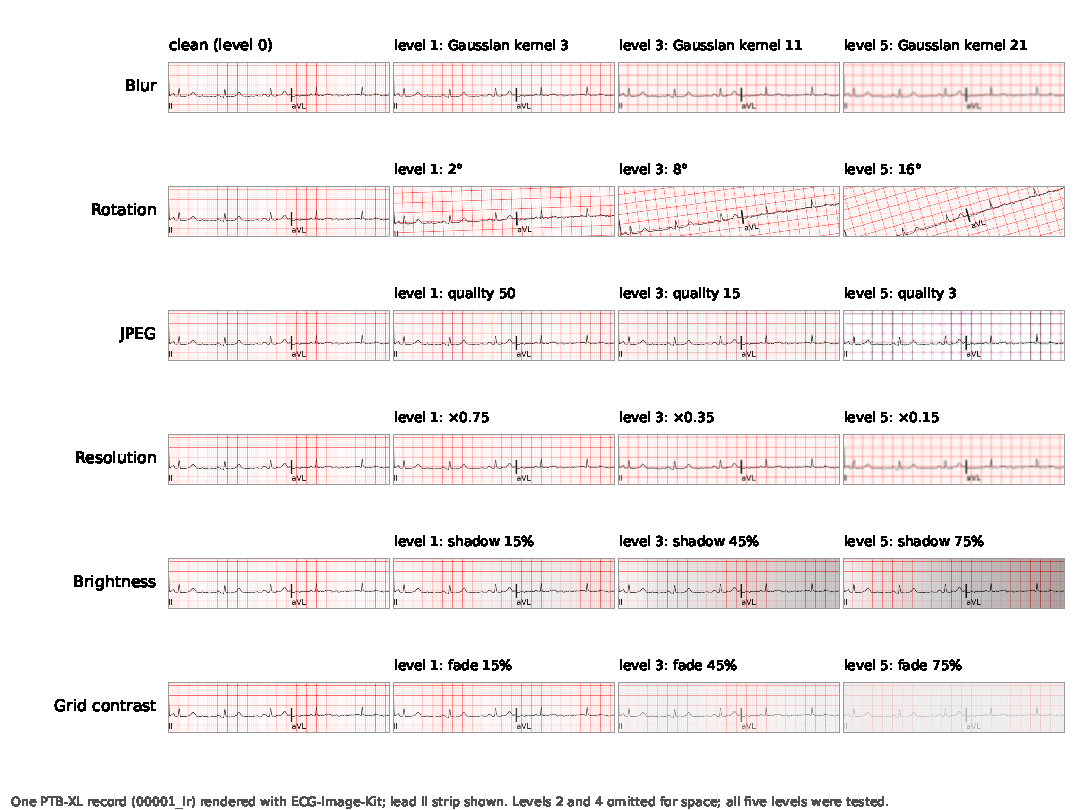
\includegraphics[width=\textwidth]{figures/fig_degradation_grid.pdf}
\caption{One real record (PTB-XL \texttt{00001\_lr}) rendered with ECG-Image-Kit and degraded exactly as in the sweep (the code that produced this figure reuses the sweep's functions). Levels 0, 1, 3 and 5 of every axis are shown, cropped to the lead~II strip; for tilt the crop follows the trace. Levels 2 and 4 were also tested.}\label{fig:grid}
\end{figure}

\subsection{Step 5: harness and pilot}
The chain was rebuilt as a notebook for Google Colab, because the local environment had by then been found to be broken (its configuration pointed at another machine's user profile). The pilot ran 10 records $\times$ blur $\times$ 6 levels (clean plus five) $=60$ tests. It served two purposes: to prove that sampling, rendering, degradation, digitisation and comparison work end to end, and to measure throughput before committing to the full sweep.

\subsection{Step 6: sweep 1 (heart rate)}\label{sec:sweep1}
Sweep~1 processed the 50-record sample $\times$ 31 versions $=1{,}550$ tests, digitising each page with Open-ECG-Digitizer and computing lead~II heart rate against ground truth. Everything that had to survive a session disconnect (the record sample, the rendered clean pages, and the results table) was stored on Google Drive. Tests were processed in sub-batches of 20; after every sub-batch the results file was written to a temporary file, swapped in atomically, copied to a time-stamped backup, and \emph{read back from Drive} with an assertion that the row count matched memory. This verified-save design was adopted after a stale browser view made a complete results file look as if $\approx$500 tests had been lost. The notebook prints the compute device at start, because newly uploaded notebooks default to CPU and this was missed three times.

\subsection{Step 7: Sweep 1 analysis}\label{sec:sweep1analysis}
Sweep~1 was analysed in Colab notebooks that read the checkpointed results file. They (i) removed duplicate and stray rows and counted unreadable tests (cleaning), (ii) identified the records that failed to digitise, separating failures on the clean image from failures caused by damage, (iii) classified each heart rate as slow ($<60$\,bpm), normal (60--100\,bpm) or fast ($>100$\,bpm) and tabulated the outcomes described in Section~\ref{sec:metrics}, and (iv) drew the figures. Records that failed to digitise were reported separately and excluded from the damage curves, leaving the reliable set.

\subsection{Step 8: sweep 2 (heart rate and intervals)}\label{sec:sweep2}
Sweep~1 discarded each digitised waveform after computing heart rate, so PR, QRS, QT and QTc could not be recovered from it. Sweep~2 therefore re-digitised every image from scratch, over the \emph{same} 50 records (same pool, same seed), and additionally extracted PR, QRS, QT and QTc from both signals (Section~\ref{sec:metrics}) and looked up patient sex for the sex-specific QTc threshold. It wrote to a separate results file so that Sweep~1's verified results could not be affected. The interval-extraction function was unit-tested on a synthetic ECG, and the full metric function was dry-run against mock ground-truth and digitised data extracted verbatim from the built notebook, before any GPU time was used.

\subsection{Step 9: Sweep 2 analysis and cross-checks}\label{sec:sweep2analysis}
Sweep~2 was analysed locally with Python scripts (Appendix~\ref{sec:repro}). They repeated the Sweep~1 analysis on the new file, added the interval error tables and the QTc outcome, and ran the cross-checks that the earlier steps had made necessary: the paired tests and Bland--Altman analysis (Section~\ref{sec:stats}), the recomputation of ground truth at 500\,Hz, the breakdown by diagnostic superclass, and a test-by-test comparison of the two sweeps.

\subsection{Metrics}\label{sec:metrics}
\textbf{Ground truth and digitised signals.} Ground truth is lead~II of the PTB-XL 100\,Hz record. The digitiser returns a 1{,}000\,Hz time series per lead in microvolts (converted to millivolts). Only lead~II was analysed. If the digitiser returned no signal, the test is a \emph{silent drop}.

\textbf{Heart rate.} R peaks were detected with NeuroKit2 and heart rate taken as the mean instantaneous rate over the record. Heart-rate error is the absolute difference between digitised and ground-truth values.

\textbf{Intervals.} After NeuroKit2 signal cleaning, R peaks were detected and P, QRS and T boundaries located with the discrete-wavelet delineator. At least three R peaks were required. PR is the mean over beats of (R-onset $-$ P-onset), QRS duration the mean of (R-offset $-$ R-onset), and QT the mean of (T-offset $-$ R-onset). QTc uses Bazett's correction with the test's own detected heart rate. As a sensitivity check on the QTc outcome analysis, Fridericia's correction (QT$/$RR$^{1/3}$) was also applied: the truly prolonged records fell from 21 to 16 and the real false-reassurance events from 6 to 2 (overlapping Wilson 95\% intervals; unchanged with a 20\,ms instead of 10\,ms tolerance), so the Bazett count is best read as an upper bound. Interval error is the absolute difference between digitised and ground-truth values. Ground-truth intervals were computed from the 100\,Hz records in the sweep and recomputed from the 500\,Hz records for the analysis in Section~\ref{sec:gt500}; intervals in the main results use the 500\,Hz version.

\textbf{Patient-facing outcome (heart rate).} A heart rate is banded as slow ($<$60\bpm), normal (60--100\bpm) or fast ($>$100\bpm) \citep{ref52}. Comparing the digitised band with the ground-truth band gives: correct; false alarm (normal truth, abnormal reading); \textbf{false reassurance} (abnormal truth, normal reading); wrong-abnormal; or silent drop. A false reassurance is counted as \emph{real} only if the digitised value is more than 10\bpm\ from the truth. A smaller discrepancy that crosses the band edge (for example 59.7 read as 60.0\bpm) is a \emph{boundary flip}, reported separately.

\textbf{Patient-facing outcome (QTc).} QTc was classed prolonged if it exceeded 460\,ms in women or 450\,ms in men \citep{ref52}, using PTB-XL sex. The same outcome categories apply, with two additions found necessary during analysis (Section~\ref{sec:qtcoutcome}): an event counts as real only if (a) it exceeds 10\,ms and (b) the same record's own \emph{clean} image was classified correctly, because a record already misclassified without any degradation cannot demonstrate a degradation effect.

\textbf{Reliable records.} A record was \emph{reliable} if the digitiser returned a heart rate for at least 25 of its 31 versions ($\le$6 unreadable, $\le$20\,\%). Degradation analyses use reliable records only; excluded records are reported separately.

\textbf{Signal-to-noise ratio.} The sweep code also computed a signal-to-noise value. We do \emph{not} report it. The computation compared the 100\,Hz ground truth and the 1{,}000\,Hz digitised signal sample by sample without resampling or time alignment, and its median on undamaged images was about $-3$\,dB, which is not meaningful. This was discovered only when preparing this paper.

\subsection{Statistical analysis}\label{sec:stats}
Errors are skewed, so we report medians with interquartile ranges (IQR) and, where a mean is informative, means. Each degraded level was compared with the \emph{same record's} clean image using a paired Wilcoxon signed-rank test, with Holm correction across the $6\times5=30$ comparisons of each metric; the effect size is the median paired excess error. Because statistical significance with 49 records can be reached for negligible effects, we always report the effect size beside it. Confidence intervals for proportions are Wilson intervals. Agreement between digitised and ground-truth values on clean images is summarised with Bland--Altman bias and 95\,\% limits of agreement. Sex-, age- and class-adjusted models were not fitted, because the number of records is too small to support them.

\section{Results}\label{sec:results}

Results are reported in the order of the steps in Table~\ref{tab:steps}. Interval errors use the 500\,Hz ground truth and 49 reliable records unless stated; heart-rate results for Sweep~1 use the 44 records that were reliable in that sweep. Sweep~1 and Sweep~2 are reported separately and compared in Section~\ref{sec:drift}.

\subsection{Steps 1--3: does the chain work at all?}

\textbf{Step 1 (stand-in renderer).} The digitiser ran in 19\,s and returned all 12 leads, but the stand-in page matched none of its known layouts, so it fell back to a default and recovered only about 2.4\,s of lead~II, in which it found two heartbeats. That is too few to give a heart rate. The recovered amplitude was about one third of the true amplitude. The result was a connectivity proof, not an accuracy result: a picture went in and numbers came out.

\textbf{Step 2 (official renderer).} With the official tool's correctly formatted page, the digitiser recognised the layout with a low matching cost (0.094), recovered the full 10\,s, found 10 beats (the true count), and gave a heart rate of 63.8\bpm\ against a true 63.9\bpm. The recovered amplitude was about 90\,\% of the true amplitude. This showed that the Step~1 shortfall came from the stand-in picture and not from the digitiser.

\textbf{Step 3 (six records).} Five of six records were digitised accurately (Table~\ref{tab:step3}, Fig.~\ref{fig:step3}): the absolute heart-rate errors were 0.02--0.21\bpm\ (mean 0.09\bpm). One record (\texttt{00002}) returned only 2.5\,s of signal and no heart rate. Its rendered page looked normal, so the failure lay inside the digitiser. The digitiser's own layout-match cost was highest for this record (0.31, against 0.09--0.23 for the five that worked). One record is far too little to conclude that this cost predicts failure, but it is the kind of early-warning signal a later quality gate would need.

\begin{table}[ht]
\centering\small
\caption{Step~3: six-record validation on undamaged rendered pages (recomputed from the saved digitiser outputs). Recovered: seconds of the 10\,s record the digitiser returned.}\label{tab:step3}
\begin{tabular}{@{}lrrrr@{}}
\toprule
Record & True HR (bpm) & Digitised HR (bpm) & Error (bpm) & Recovered (s) \\
\midrule
\texttt{00001\_lr} & 63.9 & 63.8 & 0.07 & 10.0 \\
\texttt{00002\_lr} & 47.6 & no reading & -- & 2.5 \\
\texttt{00003\_lr} & 63.7 & 63.7 & 0.02 & 10.0 \\
\texttt{00004\_lr} & 74.7 & 74.9 & 0.21 & 10.0 \\
\texttt{00005\_lr} & 66.4 & 66.5 & 0.08 & 10.0 \\
\texttt{00006\_lr} & 83.1 & 83.0 & 0.08 & 10.0 \\
\bottomrule
\end{tabular}
\end{table}

\begin{figure}[ht]
\centering
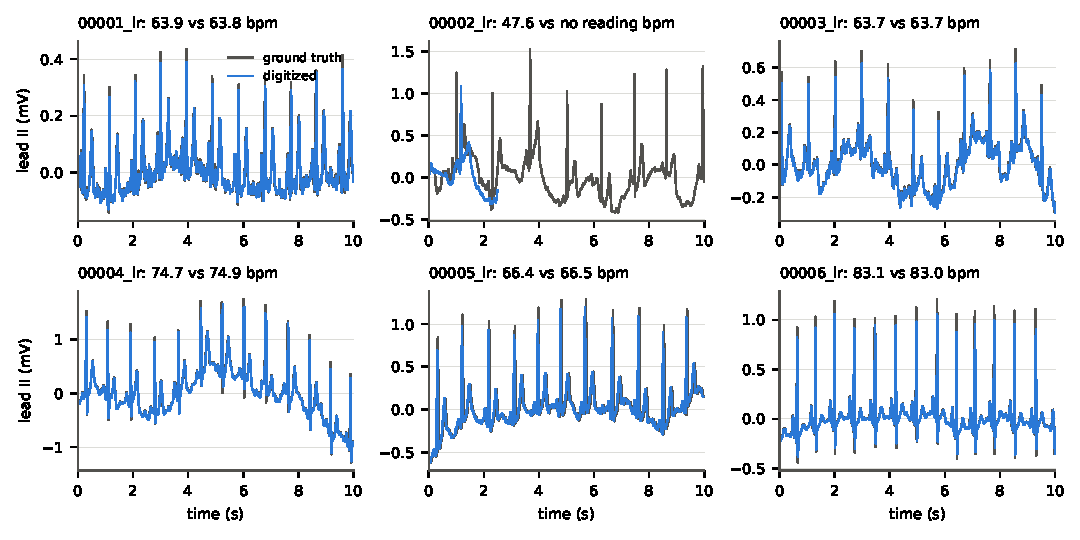
\includegraphics[width=\textwidth]{figures/fig_step3_validation.pdf}
\caption{Step~3 output: ground-truth (grey) and digitised (blue) lead~II for the six validation records on undamaged pages. Titles give true and digitised heart rate. Record \texttt{00002} shows the failure: only the first 2.5\,s were recovered.}\label{fig:step3}
\end{figure}

\subsection{Step 5: pilot}
The pilot (10 records, blur, 60 tests) ran at about 20.3\,s per image on a T4 GPU (about 120--150\,s on CPU) and showed heart-rate error rising with blur, from 0.09\bpm\ on clean images to 8.8\bpm\ at the heaviest blur in those 10 records. Its first digitiser crash (``weights only load failed'') looked like a PyTorch version problem. The cause was that \texttt{git-lfs} was not installed in the Colab image, so the model-weight files were small pointer stubs. Installing \texttt{git-lfs} before pulling fixed it. This full-sweep estimate (about 10.5 hours for 1{,}550 images) drove the scope reduction in Step~0.

\subsection{Step 6: Sweep 1 completion, cleaning and reliability}\label{sec:cleaning}
All 1{,}550 tests completed. The raw results file held 1{,}688 rows because 138 stray rows from earlier, larger scope settings had been written before the scope was reduced; after removing them there were 0 duplicates and every expected test was present. Roughly 35 minutes of progress had been made on CPU by mistake; the rest ran on a T4 GPU at 22--24\,s per image in about 5 hours. Several things went wrong along the way, each of which changed the design (Table~\ref{tab:problems}).

\begin{table}[ht]
\centering\small
\caption{Operational problems in Sweep~1 and what each changed.}\label{tab:problems}
\begin{tabularx}{\textwidth}{@{}>{\raggedright\arraybackslash}p{3.6cm}>{\raggedright\arraybackslash}X>{\raggedright\arraybackslash}p{4.4cm}@{}}
\toprule
Problem & What happened & Consequence \\
\midrule
Wrong scope ran & Step~3 copied every cached image, so the variant list covered 500 records, not 150; caught from the printed count (15{,}500 variants) & Variant list built only from the current sample \\
CPU by mistake (three times) & Newly uploaded notebooks default to CPU & Device printed and checked before trusting a run \\
GPU quota & Colab refused GPU after a few hours & Retried later; then a second account (study folder shared as editor) \\
Apparent data loss & A stale view suggested about 500 tests were lost; the file was complete & Verified saving (temporary file, atomic swap, backup, read-back check) \\
Two runs, one file & CPU and GPU runs worked on the same remaining tests and file & CPU run stopped as soon as the GPU run started \\
Hand-edited cells & Editing cells in the browser corrupted them repeatedly & Notebooks built locally, syntax-checked, dry-run on mock data, then uploaded \\
\bottomrule
\end{tabularx}
\end{table}

\textbf{Reliability in Sweep 1.} Of 1{,}550 tests, 163 (10.5\,\%) returned no heart rate, and in 154 of those no digitised signal was returned at all. The failures were concentrated in six records (unreadable in 18--31 of 31 versions: \texttt{00102}, \texttt{08150}, \texttt{13316}, \texttt{00053}, \texttt{18151}, \texttt{19059}); four of them (\texttt{00102}, \texttt{08150}, \texttt{13316}, \texttt{19059}) failed even on the clean image. Thirty-seven records never failed and seven failed once or twice (Fig.~\ref{fig:fig3}). Record \texttt{00102} also has no measurable ground-truth heart rate. These six records were excluded from Sweep~1 degradation analyses, leaving 44 reliable records.

\begin{figure}[ht]
\centering
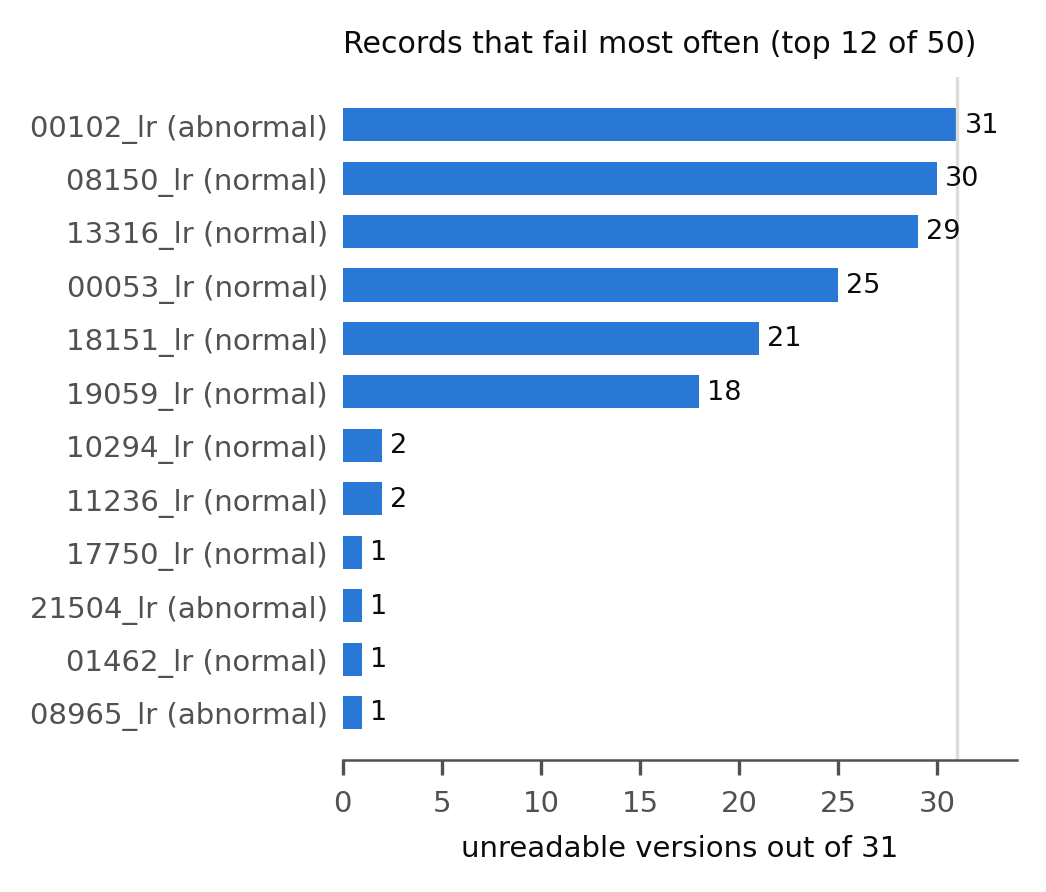
\includegraphics[width=0.55\textwidth]{figures/fig3_unreadable_records.png}
\caption{Sweep~1: the 12 records (of 50) with the most unreadable versions out of 31. Six fail in most versions, four of them on the clean image too. Sweep~2 did not reproduce this pattern (Section~\ref{sec:drift}).}\label{fig:fig3}
\end{figure}

\subsection{Step 7: Sweep 1, heart rate}\label{sec:hr1}
On clean images the mean heart-rate error was 0.52\bpm\ (median 0.13\bpm). Two of six axes showed a clear rise with severity (Fig.~\ref{fig:fig1}). For blur the mean error rose from 0.41\bpm\ (level 1) to 2.90\bpm\ (level 5), with a median of 0.12 to 1.64\bpm. For low resolution the error stayed near baseline through level~4 (median 0.11--0.20\bpm) and then jumped at level~5 to a mean of 7.72\bpm\ and a median of 2.36\bpm, with 41\,\% of readings more than 5\bpm\ off. Tilt, JPEG compression, grid contrast and uneven lighting stayed within the baseline band (mean error $\le$1.2\bpm\ at every level).

\begin{figure}[ht]
\centering
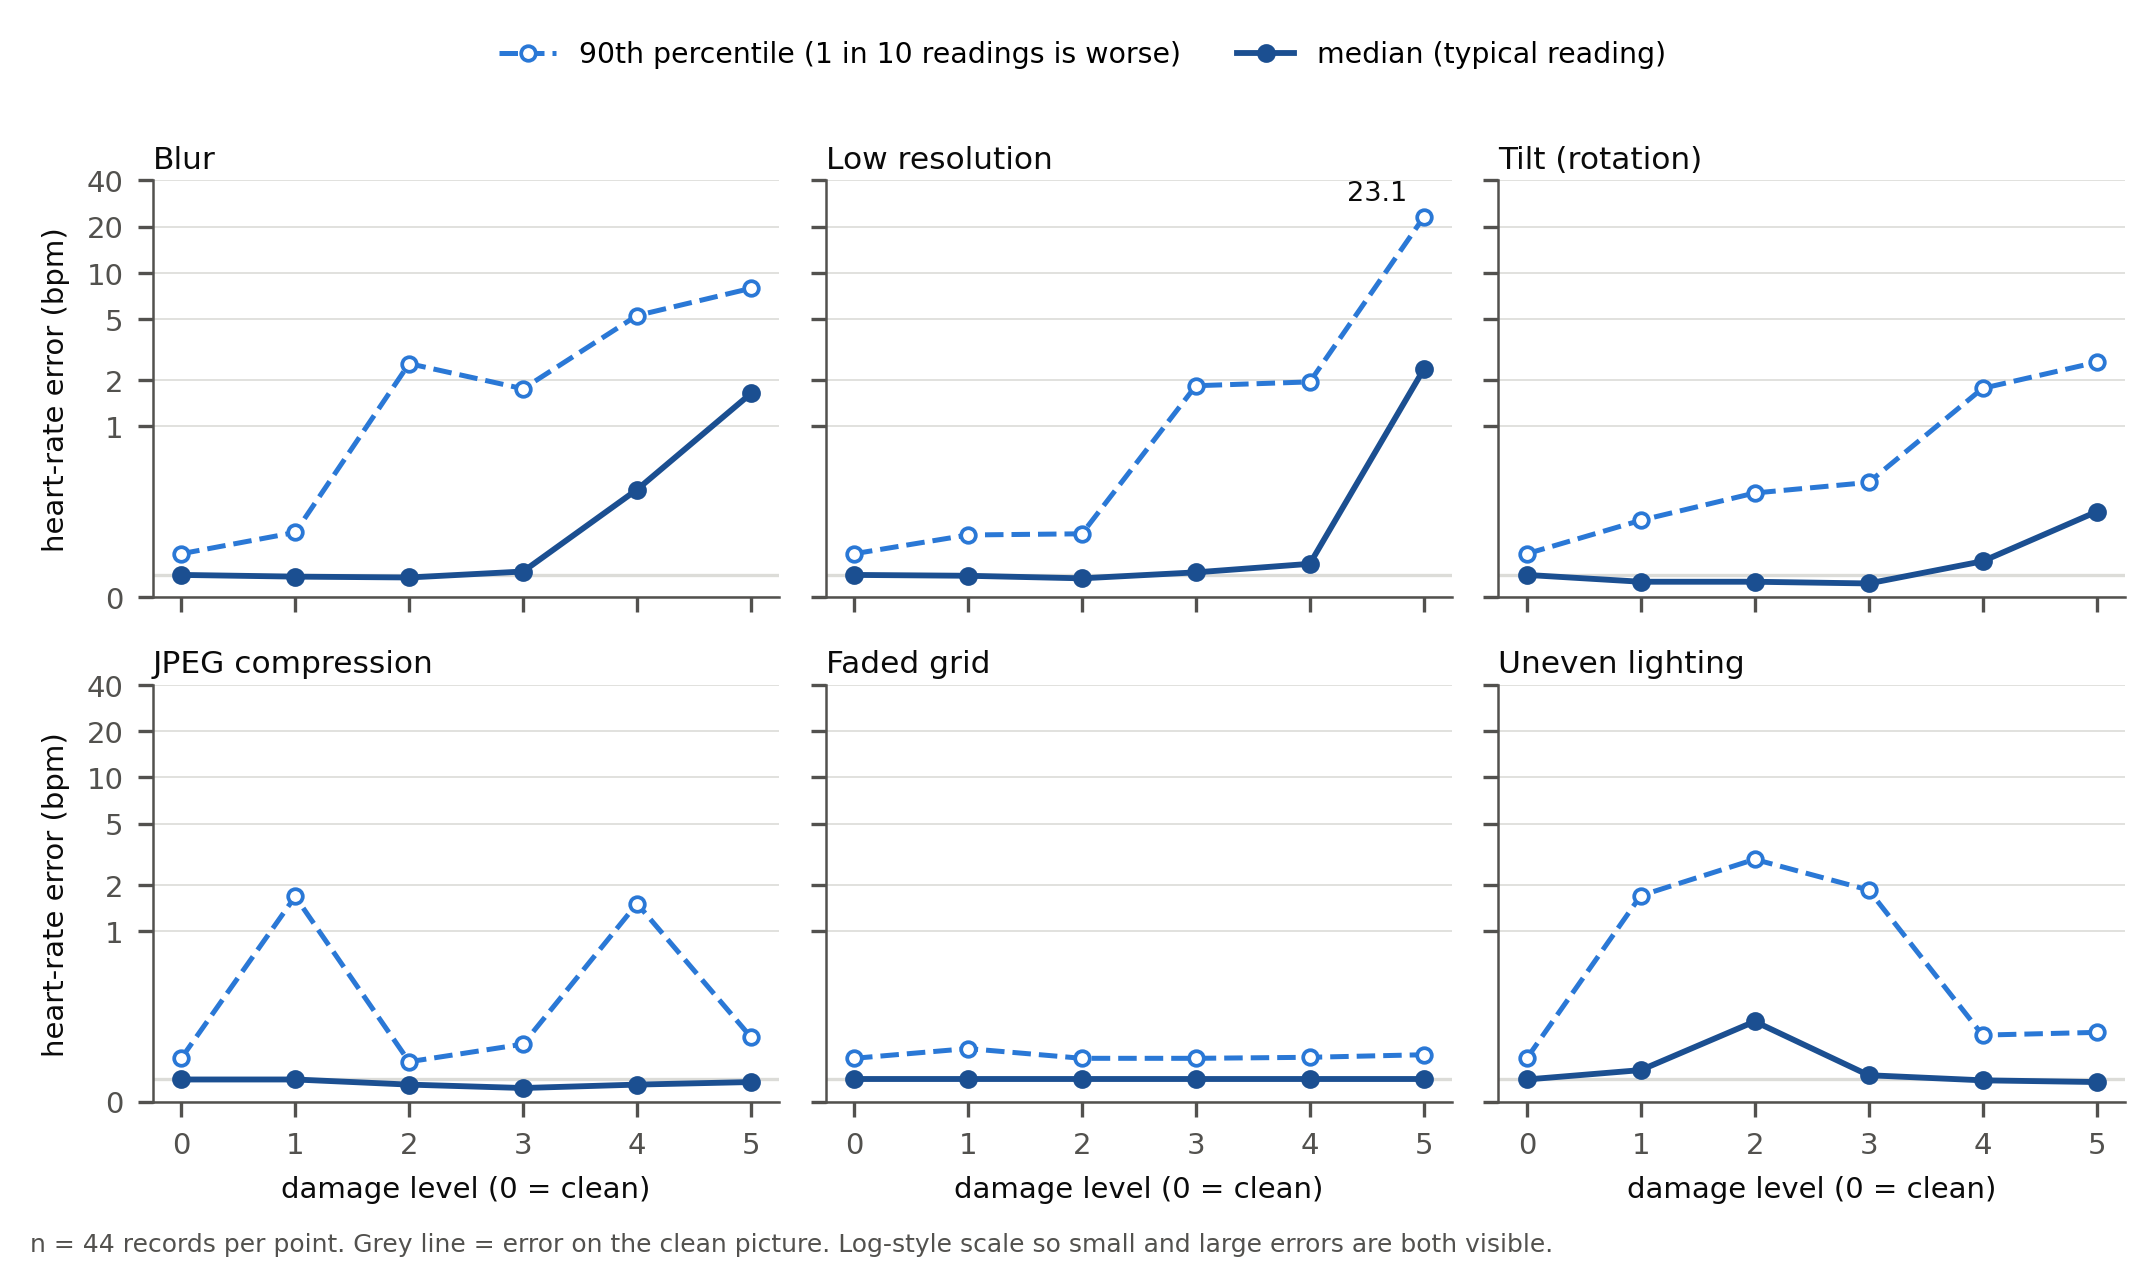
\includegraphics[width=\textwidth]{figures/fig1_hr_error_by_damage.png}
\caption{Sweep~1 (44 reliable records): absolute heart-rate error (symlog axis) against degradation level for each axis; solid line median, dashed line 90th percentile, grey line the clean-image median.}\label{fig:fig1}
\end{figure}

\textbf{Patient-facing outcome.} Only nine of the 44 reliable records have a slow or fast ground-truth heart rate (six slow, three fast) and can therefore show false reassurance. On clean images all 44 were read correctly. Across all degraded images nine readings were falsely reassuring; six were real (more than 10\bpm\ off) and three were boundary flips (for example 59.7 read as 60.0\bpm). \textbf{All six real events occurred at level~5, and only for two axes}: low resolution in 4 of 9 at-risk records (44\,\%, 95\,\% CI 19--73\,\%; errors 14--33\bpm) and blur in 2 of 9 (22\,\%, 95\,\% CI 6--55\,\%; errors about 15\bpm). No real event occurred at any other axis or at levels 1--4 of these two. Tilt caused a different failure: at level~5, 4 of 44 pictures (9\,\%) returned no reading (a silent drop) and none returned a wrong one (Fig.~\ref{fig:fig2}). With $n=9$ at risk the intervals are wide, so these counts describe a pattern, not a rate.

\begin{figure}[ht]
\centering
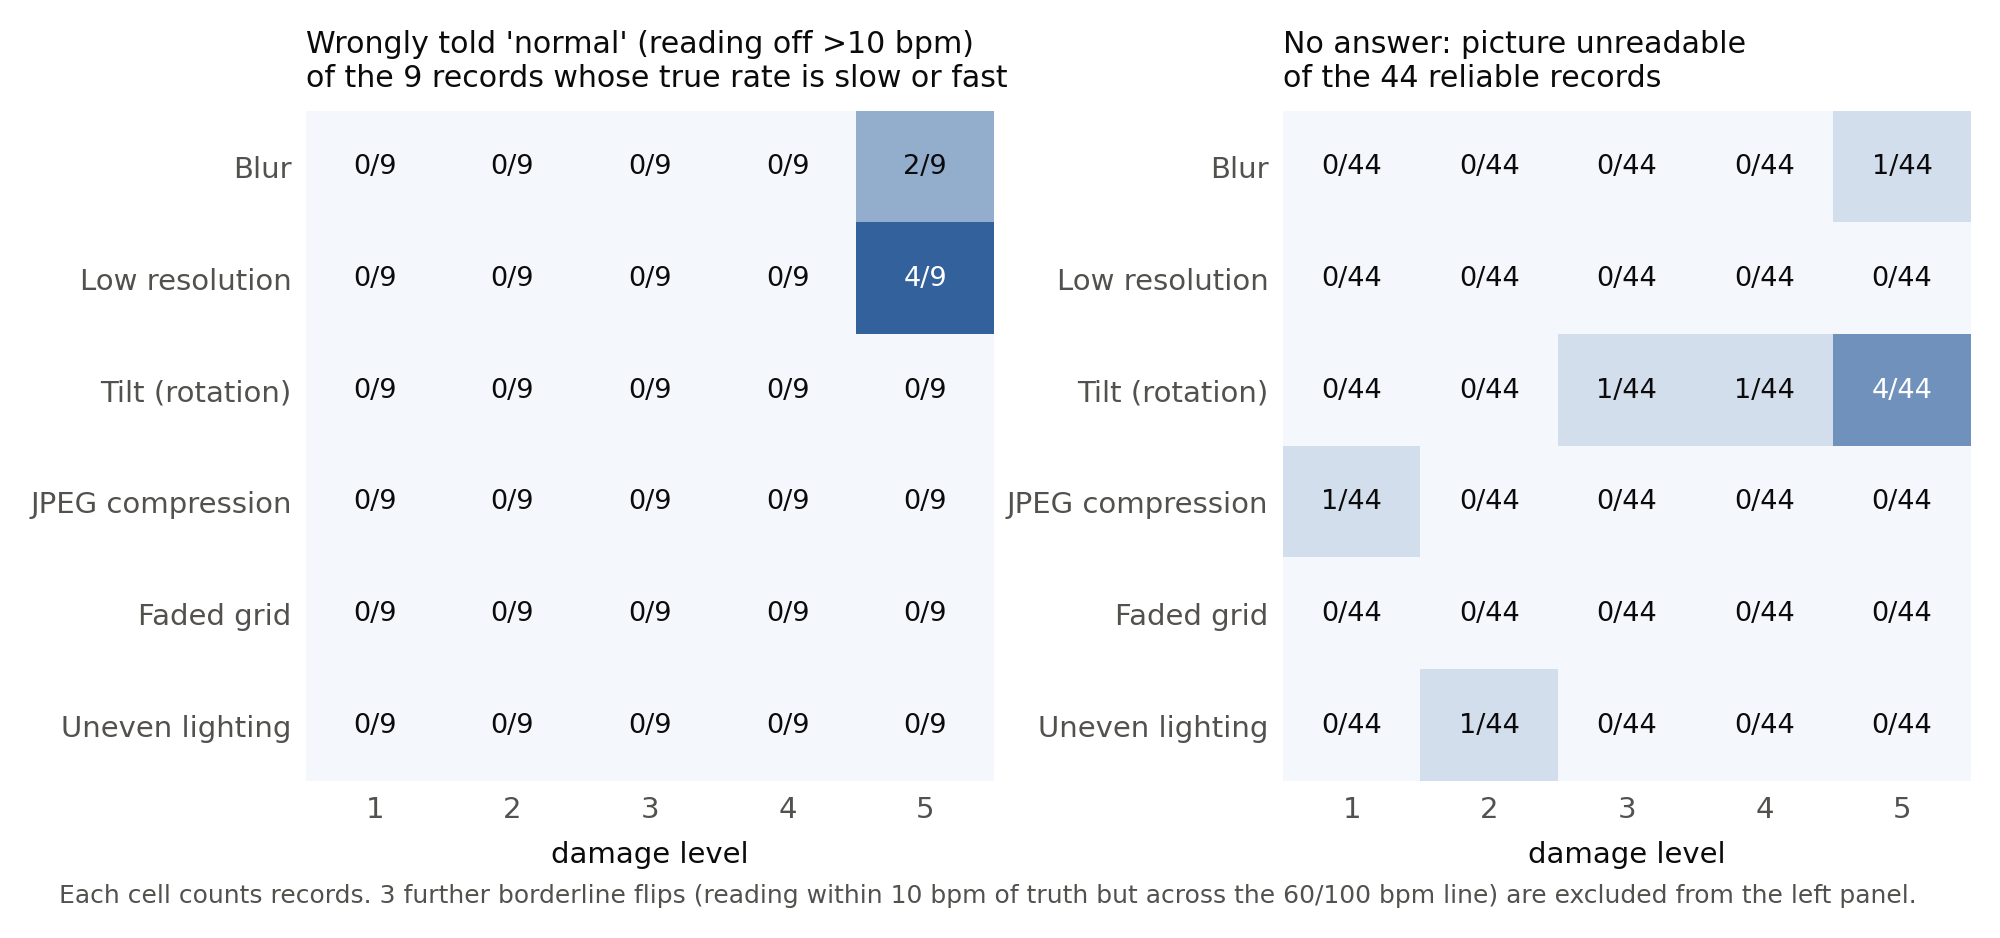
\includegraphics[width=\textwidth]{figures/fig2_false_reassurance_and_silent_drops.png}
\caption{Sweep~1. Left: of the nine records with a slow or fast true heart rate, how many were reported as normal (reading off by $>$10\bpm) at each axis and level. Right: of 44 reliable records, how many returned no reading.}\label{fig:fig2}
\end{figure}

\subsection{Step 8: Sweep 2 completion}
Sweep~2 completed all 1{,}550 tests overnight and produced a results file with 23 columns (Appendix Table~\ref{tab:dict}). Google Drive's mount misfiled checkpoint saves repeatedly: on two occasions stray copies of the results file appeared at the top level of the Drive instead of in the study folder (4 copies the first time, 19 the second). Each time, the copies were compared by row count with the file in the study folder, found to be older, smaller snapshots of the same data, and removed; no data were lost. The browser's view of the running notebook also stalled once on an accumulated-output replay problem while the kernel kept running (confirmed from Colab's session list), and was resolved by disconnecting the runtime, clearing outputs and restarting from the checkpoint. In this sweep 49 of 50 records were reliable: only \texttt{15192\_lr} failed badly (unreadable in 20 of 31 versions, but readable on its clean image). Of 1{,}550 tests, 30 (1.9\,\%) returned no heart rate and 41 (2.6\,\%) no QTc.

\subsection{Step 9: Sweep 2 analysis}

\subsubsection{Sweep 2 repeats the heart-rate findings}\label{sec:hr2}
Using the same rules as Sweep~1 on the 49 reliable records, 10 records have a slow or fast true heart rate (six slow, four fast; the fourth fast record, \texttt{08150}, was unreliable in Sweep~1). There were 10 falsely reassuring readings: \textbf{six real, all at level~5 (blur 2, low resolution 4)}, with errors of 14.2--33.3\bpm, and four boundary flips. The clean-image mean error was 0.53\bpm\ (median 0.13\bpm); at level~5 the blur mean was 3.30\bpm\ (median 1.65\bpm) and the resolution mean 7.84\bpm\ (median 2.54\bpm), with 42.9\,\% of resolution-5 readings more than 5\bpm\ off. Tilt level~5 produced 5 silent drops of 49. On the clean images, the heart-rate band matched ground truth in 48 of 49 records. The headline pattern is therefore the same in both sweeps; as Section~
ef{sec:drift} shows, this is a repeat of the same tests, not an independent replication.

\subsubsection{Agreement on clean images}
On undamaged images heart rate agreed closely with ground truth: bias $+0.26$\bpm, 95\,\% limits of agreement $-3.1$ to $+3.6$\bpm, mean absolute error 0.53\bpm\ (Table~\ref{tab:ba}, Fig.~\ref{fig:ba}). Two records (of 49) differed by more than 5\bpm. Intervals agreed much less well: mean absolute errors were 11.0\,ms (PR), 21.2\,ms (QRS), 19.3\,ms (QT) and 22.1\,ms (QTc), with systematic biases of $-7.3$, $+19.4$, $+13.3$ and $+15.4$\,ms; digitised QRS is longer than ground truth, which is consistent with a thicker reconstructed trace, although we did not test that explanation.

\begin{table}[ht]
\centering\small
\caption{Agreement on clean images (digitised minus ground truth; intervals against 500\,Hz ground truth; $n=49$ reliable records). LoA: 95\,\% limits of agreement; MAE: mean absolute error.}\label{tab:ba}
\begin{tabular}{@{}lrrrrr@{}}
\toprule
Measure & Bias & SD & LoA low & LoA high & MAE \\
\midrule
HR (bpm) & +0.26 & 1.70 & -3.1 & +3.6 & 0.53 \\
PR (ms) & -7.29 & 13.08 & -32.9 & +18.4 & 11.04 \\
QRS (ms) & +19.35 & 21.23 & -22.3 & +61.0 & 21.15 \\
QT (ms) & +13.29 & 24.77 & -35.3 & +61.8 & 19.26 \\
QTc (ms) & +15.44 & 28.02 & -39.5 & +70.3 & 22.10 \\
\bottomrule
\end{tabular}
\end{table}

\begin{figure}[ht]
\centering
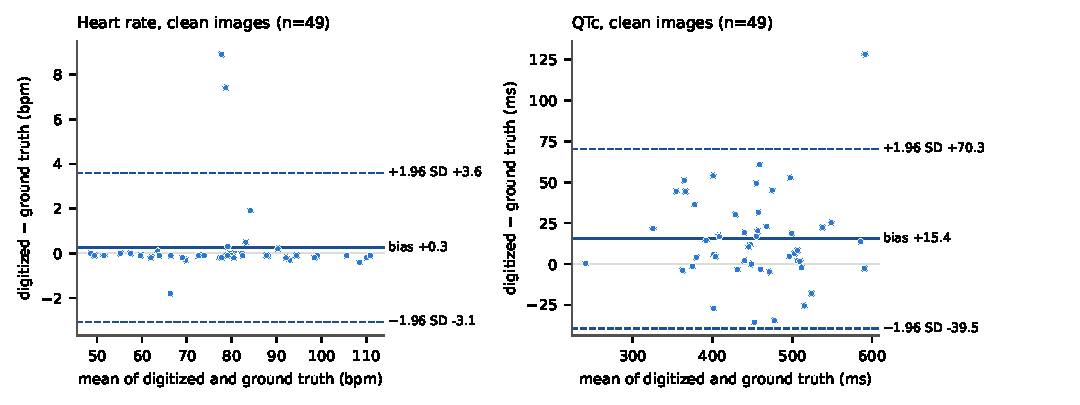
\includegraphics[width=\textwidth]{figures/fig_bland_altman_clean.pdf}
\caption{Bland--Altman plots on clean images. Left: heart rate. Right: QTc against the 500\,Hz ground truth. Solid line: bias; dashed lines: 95\,\% limits of agreement.}\label{fig:ba}
\end{figure}

\subsubsection{Interval error against degradation}\label{sec:intervalerr}
The interval results mirror heart rate (Table~\ref{tab:intervals}, Fig.~\ref{fig:intervals}). For blur, the median QTc error rose from 17.3\,ms on clean images to 24.4, 45.0, 77.8 and 90.8\,ms across levels 2--5; QRS from 16.2 to 117.6\,ms; QT from 12.9 to 77.0\,ms. For low resolution the rise was later and steeper (QTc 35.1\,ms at level 4, 73.0\,ms at level 5). \textbf{PR was the exception}: its median error rose only from 9.1 to at most 22.2\,ms and did not increase monotonically. The other four axes stayed close to the clean-image baseline (Table~\ref{tab:flat}); the largest deviation was tilt at level~5, where the median QTc error was 26.8\,ms against 17.3\,ms on clean images, which was not significant after correction.

\begin{table}[ht]
\centering\small
\caption{Median absolute error against ground truth, by level, for the two axes that matter (49 reliable records; intervals against 500\,Hz ground truth; heart rate in bpm, intervals in ms). Level 0 is the clean image.}\label{tab:intervals}
\begin{tabular}{@{}llrrrrr@{}}
\toprule
Axis & Level & HR & PR & QRS & QT & QTc \\
\midrule
Clean & 0 & 0.13 & 9.1 & 16.2 & 12.9 & 17.3 \\
\midrule
Blur & 1 & 0.12 & 9.8 & 17.7 & 14.1 & 17.3 \\
 & 2 & 0.15 & 10.2 & 34.8 & 23.3 & 24.4 \\
 & 3 & 0.16 & 16.4 & 66.5 & 40.7 & 45.0 \\
 & 4 & 0.64 & 22.2 & 107.3 & 67.9 & 77.8 \\
 & 5 & 1.65 & 16.6 & 117.6 & 77.0 & 90.8 \\
\midrule
Low resolution & 1 & 0.12 & 8.2 & 17.5 & 12.9 & 16.2 \\
 & 2 & 0.12 & 10.5 & 18.0 & 17.5 & 21.7 \\
 & 3 & 0.15 & 11.3 & 25.2 & 19.6 & 20.7 \\
 & 4 & 0.21 & 13.3 & 41.1 & 30.2 & 35.1 \\
 & 5 & 2.54 & 17.4 & 77.1 & 65.1 & 73.0 \\
\bottomrule
\end{tabular}
\end{table}
\begin{table}[ht]
\centering\small
\caption{The four axes that did not matter: lowest--highest of the five level medians of absolute error (49 reliable records). Compare the clean-image medians in Table~\ref{tab:intervals}.}\label{tab:flat}
\begin{tabular}{@{}lccccc@{}}
\toprule
Axis & HR (bpm) & PR (ms) & QRS (ms) & QT (ms) & QTc (ms) \\
\midrule
Tilt & 0.08--0.55 & 8.3--10.0 & 14.7--21.9 & 11.1--19.9 & 12.8--26.8 \\
JPEG & 0.08--0.14 & 7.3--9.1 & 15.3--18.4 & 11.6--14.0 & 12.8--16.9 \\
Grid contrast & 0.12--0.13 & 7.9--9.2 & 15.4--16.2 & 12.0--13.2 & 16.6--17.3 \\
Uneven lighting & 0.12--0.45 & 7.9--10.9 & 14.9--16.0 & 11.3--14.6 & 14.3--19.5 \\
\bottomrule
\end{tabular}
\end{table}

\begin{figure}[ht]
\centering
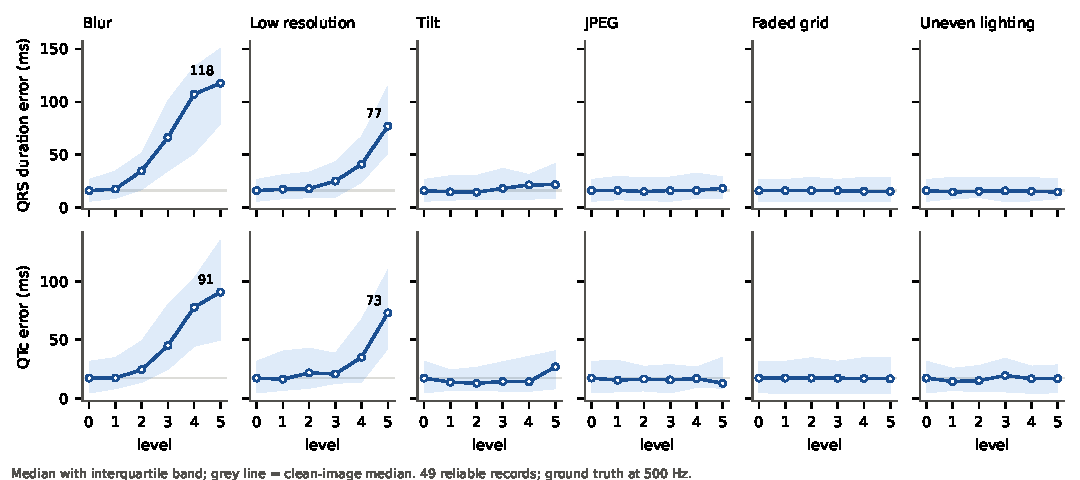
\includegraphics[width=\textwidth]{figures/fig_interval_error_by_level.pdf}
\caption{Sweep~2: QRS-duration and QTc absolute error against degradation level for each axis (median and interquartile band; grey line is the clean-image median). Numbers mark the level-5 median for the two axes that matter.}\label{fig:intervals}
\end{figure}

\textbf{Statistics.} Against each record's own clean image, blur produced significant increases (Holm-adjusted $p<0.05$) from level~2 for QRS, QT and QTc and from level~3 for PR; low resolution from level~3 for QT and QTc, level~4 for QRS and level~5 for PR (Table~\ref{tab:tests}). The effect sizes were large: at level~5, the median excess QTc error was 63.8\,ms for blur and 52.3\,ms for resolution, and the median excess QRS error 98.1 and 57.0\,ms. A few other cells were statistically significant with negligible effects, which illustrates why effect size matters: in heart rate, JPEG level~3 ($-0.03$\bpm), tilt level~4 ($+0.06$\bpm) and lighting level~2 ($+0.24$\bpm) were significant, and tilt level~5 raised QRS error by 3.9\,ms. None of these is clinically meaningful.

\begin{table}[ht]
\centering\small
\caption{Paired comparison of each degraded level with the same record's clean image (Wilcoxon signed-rank, Holm-corrected over 30 comparisons per metric). ``Lowest sig.\ level'' is the lowest level with adjusted $p<0.05$; the effect is the median paired excess error at level~5 (bpm for HR, ms otherwise).}\label{tab:tests}
\begin{tabular}{@{}llccc@{}}
\toprule
Metric & Axis & Lowest sig.\ level & Effect at level 5 & Significant cells (of 5) \\
\midrule
HR & Blur & 4 & +1.46 & 2 \\
 & Low resolution & 5 & +2.45 & 1 \\
 & Tilt & 4 & +0.31 & 2 \\
 & JPEG & 3 & +0.00 & 1 \\
 & Grid contrast & none & +0.00 & 0 \\
 & Uneven lighting & 2 & -0.01 & 1 \\
\midrule
PR & Blur & 3 & +8.01 & 3 \\
 & Low resolution & 5 & +7.23 & 1 \\
 & Tilt & none & +1.65 & 0 \\
 & JPEG & none & +0.10 & 0 \\
 & Grid contrast & none & +0.00 & 0 \\
 & Uneven lighting & none & +0.30 & 0 \\
\midrule
QRS & Blur & 2 & +98.05 & 4 \\
 & Low resolution & 4 & +57.00 & 2 \\
 & Tilt & 5 & +3.90 & 1 \\
 & JPEG & none & +2.20 & 0 \\
 & Grid contrast & none & +0.00 & 0 \\
 & Uneven lighting & none & +0.10 & 0 \\
\midrule
QT & Blur & 2 & +57.52 & 4 \\
 & Low resolution & 3 & +50.50 & 3 \\
 & Tilt & none & +3.95 & 0 \\
 & JPEG & none & +1.10 & 0 \\
 & Grid contrast & none & +0.00 & 0 \\
 & Uneven lighting & none & +0.30 & 0 \\
\midrule
QTc & Blur & 2 & +63.79 & 4 \\
 & Low resolution & 3 & +52.30 & 3 \\
 & Tilt & none & +4.30 & 0 \\
 & JPEG & none & +1.70 & 0 \\
 & Grid contrast & none & +0.00 & 0 \\
 & Uneven lighting & none & +0.17 & 0 \\
\bottomrule
\end{tabular}
\end{table}

\subsubsection{QTc patient-facing outcome (exploratory)}\label{sec:qtcoutcome}
Twenty records have a truly prolonged QTc under the sex-specific threshold. A first, naive count of falsely reassuring QTc classifications found 26 events. Twenty of these were on records whose \emph{own clean image} was already misclassified, so no degradation was needed to produce them; the interval error floor alone moved an already borderline QTc across the threshold. Counting them as degradation effects would be wrong. Requiring that the record be classified correctly on its clean image, and the error exceed 10\,ms, leaves \textbf{6 real events among 19 usable at-risk records}: blur level~2 (1), low resolution level~2 (1), tilt levels~4 and~5 (1 each), and uneven lighting levels~1 and~3 (1 each). Each cell has at most one event, so the per-cell Wilson intervals are very wide (a single event in 19 records: 5\,\%, 95\,\% CI 1--25\,\%), and the events do not concentrate at the most severe levels as the heart-rate events do. On clean images the QTc outcome was correct in 42 of 49 records, a false alarm in six and a false reassurance in one. We regard this as an exploratory, underpowered signal, not as a second confirmed false-reassurance channel.

\subsubsection{Ground truth sampling rate}\label{sec:gt500}
The sweep computed ground-truth intervals from PTB-XL's 100\,Hz records (10\,ms per sample), whereas the digitised signal is at 1{,}000\,Hz. Recomputing the ground truth from the 500\,Hz versions of the same records reduced the clean-image mean absolute error of the digitised values from 18.5 to 11.0\,ms (PR), 32.1 to 21.2\,ms (QRS), 22.7 to 19.3\,ms (QT) and 25.0 to 22.1\,ms (QTc), and the clean-image median QTc error from 20.2 to 17.3\,ms. The ground truth itself was unstable across sampling rates: for the same records, 100\,Hz and 500\,Hz ground-truth QT differed by a mean absolute 10.6\,ms, QTc by 13.2\,ms and QRS by 15.2\,ms. Even the ground-truth heart rate differed by a mean absolute 0.75\bpm\ between the two rates, which is larger than the digitiser's own clean-image heart-rate error, so heart-rate agreement is limited by ground-truth uncertainty as much as by the digitiser. The qualitative conclusions did not change with the 500\,Hz ground truth: blur and resolution still raised interval error steeply, the other axes stayed flat, and the corrected QTc analysis again gave six real events. \textbf{Part of the interval error floor is therefore an artefact of our own ground truth, and part is not.}

\subsubsection{Diagnostic superclass}
Table~\ref{tab:class} shows median errors by class. Heart-rate error was small on clean images in every class ($\le$0.2\bpm\ except the single record with no superclass), rose at level~5 of both axes in every class, and was largest under low resolution for MI (7.4\bpm, 4 records). QTc error at level~5 of blur ranged from 67 to 124\,ms across classes. Class sizes are 1--23, so no class is shown to be more or less vulnerable than another.

\begin{table}[ht]
\centering\small
\caption{Median absolute error by diagnostic superclass on clean images and at level~5 of blur and of low resolution. Classes have 1--23 records, so this is descriptive only.}\label{tab:class}
\begin{tabular}{@{}lrrrrrrr@{}}
\toprule
 & & \multicolumn{3}{c}{HR (bpm)} & \multicolumn{3}{c}{QTc (ms)} \\
\cmidrule(lr){3-5}\cmidrule(lr){6-8}
Class & Records & Clean & Blur 5 & Res.\ 5 & Clean & Blur 5 & Res.\ 5 \\
\midrule
No superclass & 1 & 7.4 & 7.7 & 11.9 & 18.0 & 61.1 & 3.5 \\
CD & 5 & 0.2 & 1.7 & 1.8 & 3.5 & 66.9 & 56.4 \\
HYP & 9 & 0.1 & 1.6 & 3.8 & 22.3 & 101.9 & 58.6 \\
MI & 4 & 0.2 & 2.9 & 7.4 & 27.7 & 99.0 & 66.0 \\
NORM & 23 & 0.1 & 1.1 & 2.9 & 19.1 & 88.3 & 82.3 \\
STTC & 7 & 0.1 & 2.0 & 0.7 & 13.6 & 124.0 & 78.5 \\
\bottomrule
\end{tabular}
\end{table}

\subsection{Reproducibility between the two sweeps}\label{sec:drift}
Sweeps 1 and 2 used the same 50 records, the same rendered pages and the same degradation code, five days apart, but an unpinned digitiser. Table~\ref{tab:repro} compares what can be compared from the recorded summaries.

\begin{table}[ht]
\centering\small
\caption{Sweep~1 against Sweep~2. Sweep~1 figures are from the recorded Sweep~1 summary; Sweep~2 figures were recomputed from its results file.}\label{tab:repro}
\begin{tabular}{@{}lrr@{}}
\toprule
 & Sweep 1 & Sweep 2 \\
\midrule
Reliable records & 44 & 49 \\
Unreadable tests (no heart rate) & 163 (10.5\,\%) & 30 (1.9\,\%) \\
Records unreadable even on the clean image & 4 & 0 \\
Records with slow or fast true heart rate & 9 & 10 \\
Real heart-rate false reassurance events & 6 & 6 \\
\quad blur, level 5 & 2 & 2 \\
\quad low resolution, level 5 & 4 & 4 \\
Boundary flips & 3 & 4 \\
Silent drops, tilt level 5 & 4 of 44 & 5 of 49 \\
Clean-image heart-rate error, mean (median), bpm & 0.52 (0.13) & 0.53 (0.13) \\
Blur level 5, mean (median), bpm & 2.90 (1.64) & 3.30 (1.65) \\
Low resolution level 5, mean (median), bpm & 7.72 (2.36) & 7.84 (2.54) \\
\bottomrule
\end{tabular}
\end{table}

We compared the two sweeps test by test, matching all 1{,}550 variants by identifier (script \texttt{v1\_v2\_per\_test\_comparison.py}, using the Sweep~1 results file). The ground-truth heart rate was identical in all 1{,}397 tests where both had one. Of the 1{,}367 tests that produced a heart rate in both sweeps, 1{,}357 (99.3\,\%) agreed to within 0.15\bpm; the other ten differed by 0.2--5.9\bpm\ (largest: \texttt{13618\_lr} at resolution level~4, 105.2 against 99.3\bpm), and on clean images the two sweeps agreed to 0.1\bpm\ or better. The same nine tilt, blur, JPEG and lighting tests were unreadable in both. The six real false-reassurance events are \emph{the same six tests} in both sweeps (\texttt{10811} at resolution~5; \texttt{15049} at blur~5 and resolution~5; \texttt{16637} at resolution~5; \texttt{20052} at blur~5 and resolution~5).

The two sweeps differed in only seven records. Six records that failed in Sweep~1 (\texttt{00102}, \texttt{08150}, \texttt{13316}, \texttt{19059}, which failed even on the clean image, and \texttt{00053}, \texttt{18151}, which failed on most versions) became readable in Sweep~2 (18--31 tests each), and \texttt{15192} went the other way (20 tests). Together these explain all 173 tests whose readable status changed. Because the digitiser was cloned afresh in each session without pinning a commit, the most likely explanation is that the upstream tool changed between the sweeps, but we cannot confirm this, because the versions were not recorded.

Two conclusions follow. First, \textbf{Sweep~2 is a repeat, not an independent replication.} The rendered pages, the degradation code and the digitiser behaviour on 43 of the records are effectively deterministic, so the same tests give the same numbers. Agreement between the sweeps shows that the pipeline is computationally reproducible; it adds no new evidence that the effect would appear on other records or images. The evidence for the effect remains that of a single 50-record sample. Second, which records fail is a property of a tool build, not of an image: a study that excludes records by name (as Sweep~1 did) is describing one build.

\section{Discussion}\label{sec:discussion}

\subsection{Two degradations matter, and the failure differs}
Across two sweeps of the same tests, only blur and low resolution produced large error growth, and only at their most severe levels did they produce a falsely reassuring heart rate. The other four axes, over the ranges tested, either did nothing measurable (JPEG compression, grid contrast, uneven lighting) or caused pictures to be unreadable rather than wrong (tilt). This distinction is practical: a system that returns nothing can ask the user to retake the photograph, whereas a system that returns a confident wrong number cannot. It also means that a quality safeguard need not treat all degradation alike.

The pattern within the interval results suggests a mechanism, which we state as a hypothesis because we did not instrument the digitiser. Blur and downscaling both smooth the trace. The narrowest feature, the QRS complex, was affected most (median error 117.6\,ms at blur level~5), QT and QTc next, and the slow P wave least (PR error did not rise monotonically). That ordering is what one expects if smoothing widens sharp features and blurs their boundaries, and it is consistent with the digitiser reconstructing a thicker trace. Tilt, by contrast, is a global geometric change that the digitiser's layout step may already correct for, and JPEG compression, lighting and grid fading alter appearance without removing the trace's edges at the severities tested.

\subsection{Where a quality gate would have to sit}
Interval error began to rise significantly at level~2 of blur and level~3 of resolution, and then rose steeply; falsely reassuring heart rates appeared only at level~5 of both. In the units of this study, level~4 of resolution is a page reduced to a quarter of its linear size and restored, and level~4 of blur is a 15\,px kernel on a page 2{,}200\,px wide. These are conditions of the simulation, not universal thresholds: a real photograph's blur and resolution depend on the camera, distance and lighting, and an operational gate would have to be calibrated on real photographs. What the results do support is the shape of the requirement: a gate should be specific to sharpness and effective resolution, need not fire on moderate tilt, compression or lighting, and cannot rely on a gradual early warning for heart rate, because under low resolution the heart-rate error is flat and then jumps at level~5.

\subsection{Interval measurements need a stated uncertainty}
Heart rate is measured robustly, with a clean-image bias of 0.26\bpm\ and 95\,\% limits of agreement of $-3.1$ to $+3.6$\bpm. PR, QRS, QT and QTc are not: on undamaged images they disagreed with ground truth by 11--22\,ms on average, with limits of agreement spanning 51--110\,ms. The prolonged-QTc thresholds (450 and 460\,ms) sit inside that band for many patients, which is why a naive count of falsely reassuring QTc classifications was inflated (26 events, 20 of them on records already misclassified on clean images). A patient-facing statement built on such a value should not carry the same confidence as one built on heart rate; it needs either a more precise delineation method or an explicit uncertainty band. This is a concrete argument for uncertainty-qualified explanation, and it is a result about the measurement, independent of the degradation.

The partial rescue from a 500\,Hz ground truth is itself informative. It shows that some of what looks like digitiser error in interval studies is ground-truth error, and that a study using a low-rate reference will overstate the error floor. It also shows the reverse for heart rate: because ground-truth heart rate differs by 0.75\bpm\ between 100 and 500\,Hz, a clean-image heart-rate error of 0.53\bpm\ cannot be interpreted as digitiser error alone.

\subsection{Reproducibility is a result, not just a hygiene issue}
The heart-rate findings came out identically in the second sweep: the same six tests were falsely reassuring, and 99.3\,\% of the tests readable in both agreed to within 0.15\bpm. This is a computational repeat, not an independent replication, because the records, pages and code were the same; it shows that the pipeline is deterministic, not that the effect would recur on new data. What did change was which records could be read: seven records changed status, including all four that failed on their clean image in Sweep~1. A study that reported only one sweep would have concluded either that four records are inherently undigitisable or that the digitiser is highly reliable; the truth is that reliability depended on the tool build. This argues for pinning tool versions, recording them, and reporting exclusions as properties of a build, not of an image.

\subsection{Relation to earlier work}
Digitisation studies commonly report signal-to-noise ratio \citep{ref2,ref5}. Our study, like the observation of \citet{ref2} that this metric does not directly reflect clinical measurements, measures clinical values instead; our own attempt to report SNR failed for a mundane reason (unaligned sampling rates), which is a small reminder of how easily a signal-level metric can be computed wrongly and go unnoticed. Quality-assessment work asks whether a signal is usable \citep{ref12,ref13,ref14}; we measure what happens downstream when it is not. And the abstention literature reminds us that declining to answer is not automatically safe \citep{ref26}. Our results suggest \emph{when} an image-quality gate might need to decline (severe blur or low resolution), but they do not test what a patient does after being asked to retake a photograph.

\subsection{What we would do differently}
(i) Pin and record every tool version from the first run. (ii) Save digitised signals from the start, so that a second, more expensive sweep is not needed for new metrics. (iii) Check the clean-image baseline of every new metric \emph{before} interpreting degradation effects; both the interval noise floor and the invalid SNR would have been seen immediately. (iv) Compute ground truth at the highest available sampling rate. (v) Align signals in time and rate before any sample-wise comparison.

\section{Limitations}\label{sec:limitations}

We state these as scope decisions and known weaknesses, in roughly decreasing order of importance for interpreting the results.

\begin{enumerate}
\item \textbf{Small sample, very small at-risk subsets.} There are 50 records; false reassurance can only arise on records whose truth is abnormal, and there are only 9 (Sweep~1) or 10 (Sweep~2) such records for heart rate and 19 usable ones for QTc. The counts show that the failure exists and where it concentrates; they are not population rates, and their confidence intervals are wide (for example 4 of 9: 95\,\% CI 19--73\,\%). The reduction from about 500 records was forced by GPU quota and time, and was decided before any result was seen.
\item \textbf{Agreement, not accuracy, for intervals.} PR, QRS, QT and QTc were obtained by applying the \emph{same} algorithm to the ground-truth signal and the digitised signal. They therefore measure agreement between two applications of one delineator, not agreement with clinician-annotated intervals, and the ground-truth QTc classification is algorithmic. The 20\,ms floor mixes digitiser error, delineator sensitivity and ground-truth sampling rate; we separated only the last.
\item \textbf{One digitiser, one renderer, one lead, simulated damage.} All results describe Open-ECG-Digitizer applied to ECG-Image-Kit pages degraded by post-processing. Real photographs combine degradations, add glare, creases, curvature and partial occlusion, and are captured by cameras with their own processing. The findings may not transfer to other digitisers or to photographs, and we make no claim that they do. Only lead~II was analysed.
\item \textbf{The digitiser was not version-pinned.} Sweeps 1 and 2 may have used different builds, and the exact versions were not recorded (Section~\ref{sec:drift}). Which records count as unreliable is therefore a property of a build, and Sweep~1's exclusions and Sweep~2's exclusions are not interchangeable. A per-test comparison showed that the sweeps agree on the 43 records readable in both (Section~
ef{sec:drift}), but this repeat shares the same 50 records, images and code, so it is not an independent replication.
\item \textbf{The QTc outcome analysis is exploratory.} It required two corrections found during analysis (excluding records already wrong on their clean image, and a 10\,ms margin), both chosen after seeing the data, and it rests on six events.
\item \textbf{Single-axis degradation.} One axis was varied at a time; real photographs vary several at once and combinations may compound.
\item \textbf{Selection by reliability.} Excluding unreliable records is a data-dependent choice; a record that fails on one build and not on another shows the choice is not neutral.
\item \textbf{Multiple comparisons and covariates.} Holm correction was applied within each metric but not across metrics, and no model adjusted for class, sex or age. Effect sizes are reported beside every significance statement for that reason.
\item \textbf{Signal fidelity was not measured.} The planned SNR tier was computed incorrectly and is not reported.
\item \textbf{Scope of the wider project.} Explanation to the patient, the safety boundary, and the application were not built or evaluated. Nothing in this paper is evidence about them or about clinical benefit.
\item \textbf{No clinical validation.} Thresholds follow published guidance for classification only. This is not a medical device and no diagnostic claim is made.
\end{enumerate}

\section{Conclusions}
In a controlled simulation of photographed paper ECGs, digitisation error was small for most degradations and large for two: severe blur and low resolution. Only these produced falsely reassuring heart rates, and they did so only at their most severe level, a result that a repeat sweep reproduced exactly (a computational repeat, not independent evidence) even though seven records changed readability. Tilt produced unreadable pictures, not wrong ones; JPEG compression, faded grids and uneven lighting did nothing measurable. Interval measurements confirmed the same pattern on top of a much larger error floor, part of which came from our own low-rate ground truth, and a QTc analogue of false reassurance was weak and not concentrated. Two lessons extend beyond this study: measure a new metric's clean-image baseline before interpreting degradation effects, and pin and record tool versions. The next steps are a version-pinned re-run on more records, a more precise interval delineation with explicit uncertainty, real photographs, a second digitiser, and only then the explanation and safeguard stages that motivated the work.

\subsection*{Work started after this manuscript}
Since this study was written up, a first step on the image-quality proxy named above as future work has begun, and is recorded here for completeness even though it was not part of the design of the study reported above and was not subject to its pre-registered scope decisions. Five signals computable from a photograph alone (no ground truth, no digitiser internals) were implemented: Laplacian-variance blur, a Hough-line-based skew estimate, an FFT high-frequency-energy resolution estimate, global intensity contrast, and a spectral JPEG-blockiness measure. On a small spike test (six demonstration pages, not the 50-record study sample, degraded with the same code used to build this study's images), every signal moved monotonically with its targeted degradation axis (Spearman $|\rho|$ 0.88--0.98 against level). Two needed correction before they worked: the skew estimate initially locked onto the ECG trace's own curved edges rather than the page's straight structural lines, fixed by requiring candidate lines to span at least 30\,\% of the image width; and the blockiness measure's first, spatial version was unusable noise, replaced by a spectral one that is monotonic but moves opposite to the naive expectation (weaker signal, not stronger, as JPEG damage increases), for a reason not yet established.

The five signals were then computed for all 1{,}550 images of the present study (not the six-page spike sample) and compared against the results already reported above, rather than left as an untested proposal. Four of the five correlated with the real measured QRS-duration error (Spearman, matched on 1{,}509 of 1{,}550 tests): blur ($\rho=-0.306$, $p=3.4\times10^{-34}$), resolution ($\rho=-0.285$, $p=1.2\times10^{-29}$), contrast ($\rho=-0.260$, $p=1.2\times10^{-24}$) and blockiness ($\rho=+0.085$, $p=9.1\times10^{-4}$); skew did not ($\rho=-0.020$, $p=0.47$). The two strongest correlations, blur and resolution, are the same two axes this study found to matter for both heart rate (Section~\ref{sec:hr1}) and intervals (Section~\ref{sec:intervalerr}), obtained here independently from measured error rather than assumed from the design. Using the same false-reassurance definition, the same 49 reliable records and the same 19 usable at-risk records (589 individual tests) reported in Section~\ref{sec:qtcoutcome}, a logistic-regression classifier fit on all five signals reached an AUC of 0.785 against the same six real events reported there -- the independent recomputation reproduced that count exactly, which is itself a check on both analyses. That AUC of 0.785 was, however, fit and evaluated on the same 589 tests it was trained on, with no held-out split, and rests on only six events, so it is optimistic and is not reported as a held-out result. A stricter follow-up held out whole recordings (49 recordings, 1{,}519 tests, repeated five-fold, cluster-bootstrap interval) and widened the target to any reading that was unreadable or wrong by more than a fixed tolerance. For heart rate off by more than 5\,bpm (99 bad readings) the five signals reached an AUC of 0.607 (95\% interval 0.49--0.82), against 0.655 for an oracle told the exact damage type and level; for larger errors the result was stronger (heart rate $>$10\,bpm 0.825, QTc $>$60\,ms 0.767, QRS $>$100\,ms 0.736). Training without one damage type and testing on it gave AUCs of 0.32--0.37 for brightness, JPEG and rotation, so the detector does not yet generalise to damage it was not built around. It is therefore reported as a promising prototype, not a working detector.

\section*{Data availability}
PTB-XL is public (PhysioNet; CC-BY~4.0) \citep{ref45}. The 1{,}550-row results tables of both sweeps, the analysis scripts, the notebook-builder scripts and the figures are in the project repository. \todo{deposit them in a public archive (for example Zenodo) and give the DOI; the repository is not currently public}. ECG-Image-Kit \citep{ref1} and Open-ECG-Digitizer \citep{ref5} are public; the exact versions used were not recorded (Section~\ref{sec:drift}).

\section*{Ethics}
No new data from human participants were collected. The study used a publicly released, de-identified dataset under its licence. \todo{confirm with the institution whether a formal ethics determination or exemption statement is required}.

\section*{Use of AI assistance}
\todo{Decide and state, in line with IOP's policy on AI tools, the extent to which an AI coding and writing assistant was used. It was used extensively in this project for code, analysis and drafting, and every number, citation and claim must be checked by the authors before submission.}

\section*{Funding, competing interests, author contributions, acknowledgements}
\todo{to be completed by the authors}


\bibliographystyle{apalike}
\bibliography{references}

\appendix
\section{Supplementary material}

\subsection{Reproducing the study}\label{sec:repro}
Everything below is in the project repository. Run in this order.

\begin{enumerate}
\item \textbf{Environment.} Python~3.11 with ECG-Image-Kit's core requirements (handwriting extras omitted); Python~3.13+ with NumPy, SciPy, pandas, Matplotlib, OpenCV, \texttt{wfdb}, NeuroKit2 for analysis; Google Colab (T4) for digitisation. \emph{Record the commit of every tool at the start of each run} (not done in this study).
\item \textbf{Sweep 1.} \texttt{colab/MediSense\_Cardio\_FullSweep\_v1.ipynb} (built by \texttt{scripts/notebook\_builders/build\_fullsweep\_notebook.py}). Set the runtime to T4 GPU, confirm the log prints \texttt{Using device: cuda}, and run all; it resumes from \texttt{results.csv} on Drive.
\item \textbf{Sweep 1 analysis.} \texttt{colab/MediSense\_Cardio\_Analysis\_Part1.ipynb} (cleaning), \texttt{Part1b} (failing records), \texttt{Part2} (heart-rate outcomes), \texttt{Part3\_figures}.
\item \textbf{Sweep 2.} \texttt{colab/MediSense\_Cardio\_FullSweep\_v2\_Intervals.ipynb}, writing \texttt{results\_v2.csv}.
\item \textbf{Sweep 2 analysis (local).} \texttt{scripts/analysis/analyze\_v2\_intervals.py} (cleaning, intervals, QTc outcome), \texttt{hr\_outcomes\_v2.py}, \texttt{check\_gt\_sampling\_rate.py} and \texttt{redo\_intervals\_gt500.py} (500\,Hz ground truth), \texttt{journal\_extra\_analysis.py}, \texttt{journal\_tables.py}, \texttt{journal\_latex\_tables.py}.
\item \textbf{Figures.} \texttt{journal\_fig\_degradation\_grid.py}, \texttt{journal\_figs\_results.py}; Sweep~1 figures from \texttt{Part3\_figures}.
\end{enumerate}

\subsection{Results file data dictionary}
\begin{longtable}{@{}>{\ttfamily}p{3.6cm}p{11.2cm}@{}}
\caption{Columns of the Sweep~2 results file (\texttt{results\_v2.csv}, 1{,}550 rows).}\label{tab:dict}\\
\toprule
Column & Meaning \\
\midrule
\endfirsthead
variant\_id & Unique test identifier: record, axis and level (for example \texttt{15049\_lr-0\_\_blur5}). \\
record & PTB-XL record name. \\
axis & \texttt{clean}, \texttt{blur}, \texttt{rotate}, \texttt{jpeg}, \texttt{resolution}, \texttt{brightness} or \texttt{gridcontrast}. \\
level & 0 (clean) or 1--5. \\
sex & \texttt{male} or \texttt{female}, from PTB-XL metadata. \\
gt\_hr & Ground-truth lead~II heart rate (bpm), from the 100\,Hz record. \\
gt\_pr\_ms, gt\_qrs\_ms, gt\_qt\_ms, gt\_qtc\_ms & Ground-truth intervals (ms) from the 100\,Hz record (the analysis recomputes them at 500\,Hz). \\
gt\_qtc\_abnormal & Ground-truth QTc above the sex-specific threshold. \\
dig\_hr, dig\_pr\_ms, dig\_qrs\_ms, dig\_qt\_ms, dig\_qtc\_ms & Values from the digitised signal; empty if none could be extracted. \\
dig\_qtc\_abnormal & Digitised QTc above the sex-specific threshold. \\
diff\_bpm, diff\_pr\_ms, diff\_qrs\_ms, diff\_qt\_ms, diff\_qtc\_ms & Absolute difference between digitised and ground-truth values. \\
snr\_db & \textbf{Invalid; do not use} (Section~\ref{sec:metrics}). \\
\bottomrule
\end{longtable}

\subsection{Digitiser configuration}
Key settings passed to Open-ECG-Digitizer in both sweeps: segmentation U-Net weights \texttt{unet\_weights\_07072025.pt} (4 output channels, 8 stages, depth 2); lead-name U-Net \texttt{lead\_name\_unet\_weights\_07072025.pt}; layout file \texttt{lead\_layouts\_george-moody-2024.yml}; \texttt{target\_num\_samples} 10{,}000; \texttt{resample\_size} 3{,}000; dewarping off; perspective detector 250 angles; pixel-size finder 30--70 grid lines. The full generated configuration is in the sweep notebooks.

\subsection{Corrections made while preparing this manuscript}
For transparency, the following were found and corrected during preparation, and are recorded so that readers of earlier drafts know what changed.
\begin{itemize}
\item The planned SNR tier was found to be computed on unaligned signals and was removed.
\item A first attribution of the interval error floor to delineation alone was revised after the 500\,Hz ground-truth check.
\item A first QTc false-reassurance count of 39 (100\,Hz ground truth) or 26 (500\,Hz) was found to be dominated by records already misclassified on their clean image, and was corrected to 6.
\item An earlier draft labelled a mean as a 90th percentile; several citations were re-assigned after re-checking the reference list against the sources.
\item A patient age of 300 in PTB-XL was recognised as a de-identification code.
\end{itemize}


\end{document}
